\chapter{Introdución}\label{cap:intro}

En este trabajo se va a estudiar el proceso de diseño de un bloque fundamental
en cualquier sensor de imagen CMOS, el canal de lectura, que es el encargado
de convertir la información física recibida, que en esencia es el número de fotones
captados por cada píxel, a una señal electrónica analógica que posteriormente será digitalizada,
procesada y, eventualmente, almacenada.\\

El estudio se va a centrar principalmente en el layout de este canal de
lectura y en todos los aspectos a tener en cuenta a la hora de abordar esta tarea.
El layout de un sistema microelectrónico consiste en su implementación física
sobre una oblea de algún material semiconductor, típicamente silicio cristalino. El
diseño de layout está sujeto a una serie de normas y problemas que iremos tratando
con mayor detenimiento a lo largo de la exposición.\\

Para introducir al lector en la materia será necesario describir, aunque sea
brevemente, conceptos sobre sensores de imágen, tecnología CMOS y explicar de manera
sencilla la arquitectura de un canal de lectura habitual.\\

Posteriormente se pasará a analizar en detalle los problemas y cuestiones que se
plantean a la hora de diseñar el layout de bloques analógicos en general,
centrándonos en última instancia en los que afectan directamente a un canal de lectura.\\

\section{Sensores de imagen}\label{cap:image_sensors}

Un sensor de imagen o cámara fotográfica es, en esencia, un sistema que capta
una imagen instantánea de una escena mediante la luz que emiten los objetos que
se encuentran en su campo de visión y que llegan a una pantalla donde se almacena
la información que proyecta ese rayo de luz, ya sea por un proceso químico
o bien electrónico, que es el caso que se va a tratar aquí.\\

En cuanto a los sensores de imágenes electrónicos se pueden distinguir dos tipos
principalmente, los CCD (\textit{Charge-Coupled Device}) y los CMOS
(\textit{Complementary Metal-Oxide-Semiconductor}). Las diferencias entre ellos
se basan en la tecnología empleada y en la forma de leer el array de píxeles.
\cite{Moini2010}\cite{Nakamura2005}\\

\paragraph{Sensores de imágen CCD}
El concepto fundamental de un sensor de imagen CCD se basa en el almacenamiento
y propagación de los electrones fotogenerados en cada píxel. Mediante el efecto
fotoeléctrico, un fotón que impacte en la zona de silicio fotosensible, si tiene
la energía adecuada, arrancará un electrón desde la banda de valencia hasta la
banda de conducción, y podrá moverse libremente o arrastrado por campos eléctricos.\\

La carga almacenada en cada píxel será función lineal de la intensidad lumínica
captada. Tras la exposición, las cargas almacenadas en cada uno de ellos
se irán transmitiendo al píxel inferior, y, de la misma forma que ocurre en un
registro de desplazamiento, la información de todos los píxeles se va transmitiendo
de unos a otros, hasta que al final todo el array es leído.\cite{Nakamura2005}\\

\paragraph{Sensores de imágen CMOS}
La diferencia fundamental de éstos con los sensores CCD es que los CMOS usan un
amplificador integrado en el píxel, a lo que nos referimos como APS (\textit{Active Pixel Sensor})
\cite{Fossum1993}. Ésto les da algunas ventajas
frente a los CCD, por ejemplo, sufren de menor efecto de ``blooming'', que podría
traducirse como deslumbramiento o destello, es decir, manchas blancas que pueden
producir los puntos muy brillantes a su alrededor por un desbordamiento de los
electrones fotogenerados en una zona. Podemos ver un ejemplo en la
imágen \ref{fig:blooming}.\\

\begin{figure}[h]
	\centering
	
\includegraphics[width=0.6\textwidth]{img/blooming.jpg}
	\caption{Ejemplo de imágen con efecto de \textit{blooming} en los píxeles brillantes
	\protect\footnotemark}
	\label{fig:blooming}
\end{figure}

Otra ventaja es que pueden llegar a ser más rápidos y más baratos, ambas debidas
al uso de la tecnología CMOS. Gracias a esto, hoy en día cada vez son más comunes que los
CCD.\\

\footnotetext{Imágen de Wikimedia Commons\cite{Commons:Kriplozoik}}

\section{Arquitectura de sensores de imagen CMOS}

\subsection{Array de píxeles}\label{cap:pxa_array}

El dispositivo principal en un sensor de imagen es el píxel, que es el elemento
receptor de la luz y el encargado de hacer la primera conversión de fotones a
electrones. Estos fotones se traducen en electrones por medio del efecto fotoeléctrico
descrito por Albert Einstein: cada fotón que incida en la superficie del silicio
es capáz de dar la energía suficiente a un electrón de la banda de valencia para que
pase a la banda de conducción y se pueda mover libremente por la red cristalina.
Si ahora aplicamos un campo eléctrico podemos guiar a todos los electrones
fotogenerados hacia un pozo de potencial donde almacenarlos temporalmente. Este
es el llamado proceso de exposición, que tiene una duración definida. En función
del tiempo de exposición y de la intensidad lumínica recibida por el píxel, este
se cargará con mayor o menor número de electrones.\\

El array de píxeles es la matriz compuesta de todos los píxeles organizados en filas
y columnas dónde la imagen formada por el sistema de lentes focalizará la imagen.
Habitualmente, los píxeles son cuadrados con un lado de unas 5 a 10 $\mum$, y el
array puede tener resoluciones de miles de píxeles en ambas dimensiones, lo que
significa que el array puede unos ocupar pocos centímetros, lo que lo convierte
habitualmente en el bloque más grande de todo el diseño.\\

En éste estudio vamos a trabajar con un array QSXGA de 2560 columnas por 2048 filas,
que tiene una relación de aspecto 5:4. Además de los píxeles activos, en un sensor
de imagen, habitualmente se incluyen algunos píxeles dummy, esto es, que no van
a ser incluidos en la imagen leída. Su función es la de evitar que los píxeles
en el borde tengan un entorno diferente al resto de píxeles del interior, lo que
puede alterar sus características.\\

Además de los píxeles dummy, habitualmente se incluyen algunos de los llamados
píxeles oscuros, píxeles iguales a los activos salvo que, por construcción no
reciben luz. Ésto se hace tapando el fotodiodo con los metales superiores,
sin modificar el resto de estructuras y transistores. El objetivo de estos píxeles
oscuros es ayudar en la calibración de los sensores una vez fabricados. Si
leemos píxeles que están tapados obtenemos el verdadero valor de negro y podemos
cuantificar el ruido debido exclusivamente al generado por el píxel y el canal,
independientemente de las condiciones externas.\\

\begin{figure}[h]
	\centering
	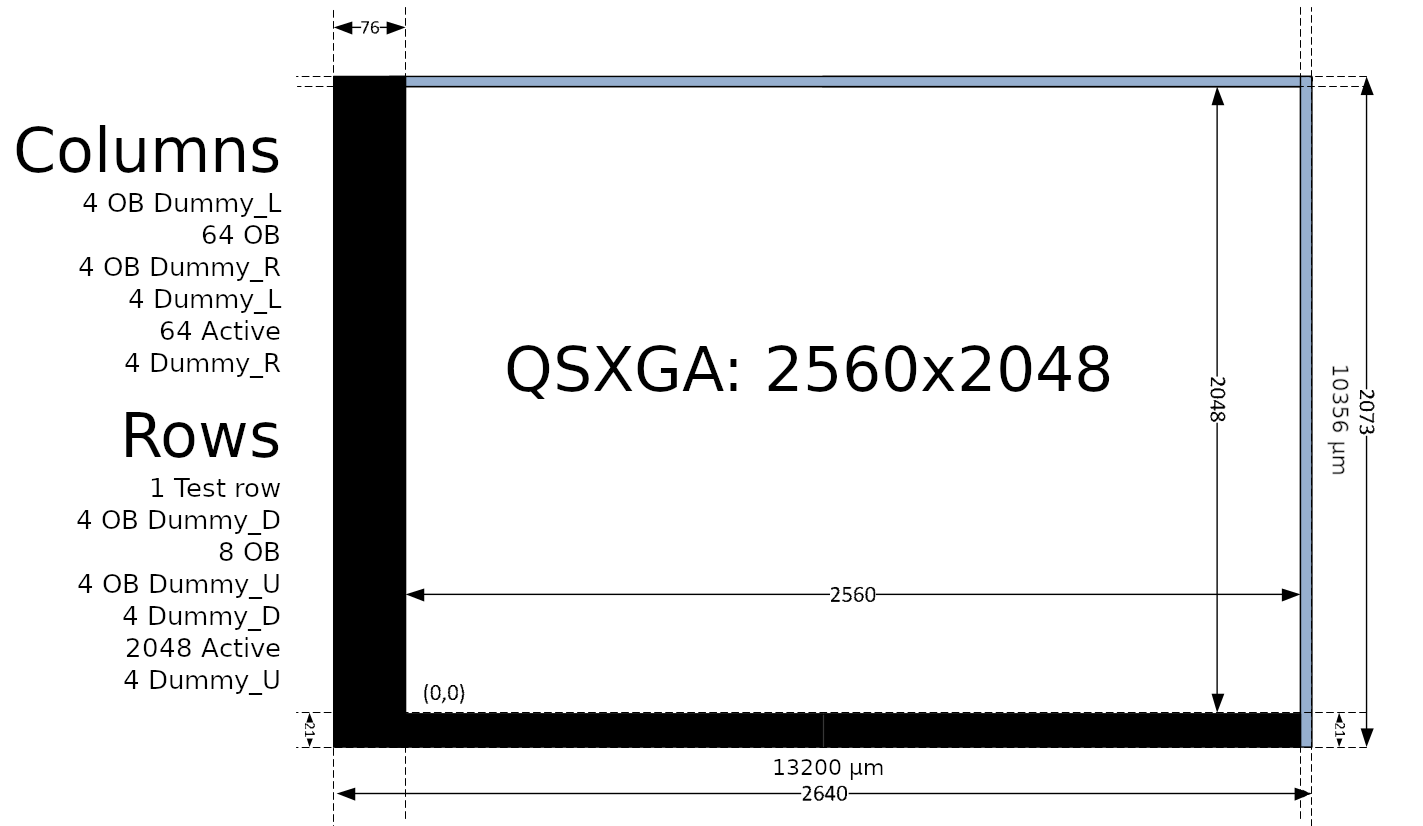
\includegraphics[width=0.9\textwidth]{img/pixel_array.png}
	\caption{Estructura del array de píxeles\protect\footnotemark}
	\label{fig:pxa_array}
\end{figure}
\footnotetext{Imágen obtenida del artículo de la bibliografía \cite{Jimenez-Garrido2012}.
Medidas en píxeles, y en $\mum$}

El sensor que estamos estudiando tiene $2560\times2048$ píxeles activos, 64 columnas
oscuras, con 4 píxeles dummy a cada lado de los píxeles activos y oscuros.
En cuanto a las filas, tendremos 8 filas oscuras en la parte inferior del array,
flanqueadas por 4 filas dummy arriba y abajo, al igual que alrededor de las filas
activas. Además se incluye una fila de test que servirá para la calibración simulando
que la fila en cuestión ha recibido una señal concreta. En la figura
\ref{fig:pxa_array} se esquematiza la estructura del array.\\

\subsection{Canal de lectura}

El canal de lectura de un sensor CMOS, referido habitualmente por sus
siglas en inglés \textbf{RO} (\textit{Read-Out Channel}), es el bloque que se
encarga de traducir el voltaje almacenado en cada píxel durante el proceso
de exposición, en un número digital. Esta descripción concuerda con el concepto
ampliamente utilizado en electrónica de ADC, siglas en inglés de \textit{Analog-to-Digital
Converter}, (Convertidor Analógico-Digital), que, en general toma una señal
analógica y la expresa en valores discretizados.\\

\subsection{Otros bloques}

\paragraph{Ana ctrl row} Este bloque se encarga del control analógico de las
señales que excitan el array por filas. Se sitúa a la izquierda y/o derecha del
array.

\paragraph{vddpix (Pixel supply)} Es el bloque anaólgico que se sitúa en la parte superior
del array de píxeles y que provee la alimentación del array
y en ocasiones también provee señales que se distribuyan de forma vertical.

\paragraph{Referencias} Es un bloque que se encarga de generar tensiones y corrientes
de polarización para el resto de bloque de forma que sean independientes de la
temperatura, fuente de alimentación y otros ruidos.

\paragraph{SPS o serializador} En el bloque digital que se encarga de ordenar en frames y serializar
los datos de salida del canal de lectura para que puedan ser enviados al exterior del
chip por los puertos LVDS de salida en serie.

\paragraph{SCM o Control Main} Es el bloque digital encargado del control de todas las
señales y procedimientos que el sensor debe realizar para tomar una imágen, digitalizarla,
y enviarla al exterior.

\paragraph{SCB} Es el bloque digital de registros donde se guardan las configuraciones
que hacen hacen funcionar el sensor de una forma especificada por el usuario.

\paragraph{SSH} Es el bloque digital que genera las señales digitales de control
del array por filas, que se pasan al \textit{ana ctrl row} para ser bufereadas hacia el array.\\[1cm]

\begin{figure}[h]
	\centering
	\includesvg[width=\textwidth]{svg/sensor_floorplan.svg}
	\caption{Floorplan aproximado del chip completo con los bloques más importantes\protect\footnotemark }
	\label{fig:floorplan}
\end{figure}

\footnotetext{Imagen trabajo propio}
%\vfill
